\chapter{Calibration}
\label{ch:calibration}


The digital readouts from the TDC and ADCs representing PMT signals
must be converted into physically-relevant quantities.
The TDC values represent hit times of PMTs,
and the ADCs represent the charge collected by the PMTs,
which ultimately must be traced back to the energy deposited
in the liquid scintillator of the ADs.
The conversion factors for these quantities were determined
through the calibration process.

Calibration ensured that the energies, times, and positions
reported by the ADs were accurate,
allowing for an unbiased and precise measurement
of the oscillation parameters.
The \thetaot{} measurement depends on well-understood detection efficiencies.
Since the IBD selection involves cuts on both energy and position,
the AD-to-AD variation in these efficiencies can be minimized
by an effective calibration.
The energy calibration was more directly critical to the measurement
of \dmsquared{}, as evidenced by the appearance of $\dmsquared/E$
in the survival probability formula, \cref{eq:p_sur_ee},
but a consistent energy response across ADs
was also important for ensuring similar selection efficiencies
in the \thetaot{} analysis.

Multiple sources were used to calibrate the ADs.
Automated calibration units were designed to deploy radioactive sources
and LEDs into the ADs.
Spallation neutrons produced by cosmogenic muons
generated a sizeable clean sample of neutron captures
on both gadolinium and hydrogen.
Single photoelectron (SPE) dark noise within the PMTs
was used to calibrate their gains.
Lastly, the energy spectrum of single (isolated) events
contained many identifiable $\alpha$ and $\gamma$ peaks,
which were used to calibrate the energy response at a wide range of energies.
\Cref{sec:acus} describes the automated calibration units.
The energy calibration consisted of multiple sub-calibrations,
described in \cref{sec:gain,sec:light_yield_calib}.
The timing calibration is described in \cref{sec:time_calib}.
Special calibration runs were performed in addition to
the weekly and continuous calibrations;
those special calibrations are described in \cref{sec:special_calib}.
Assessments of the channel quality are discussed in \cref{sec:channel_quality}.

\section{Automated calibration units}
\label{sec:acus}

The calibration system for the Daya Bay ADs
allowed for automated deployment of a variety of calibration sources.
Each AD was outfitted with three automated calibration units (ACUs)
which could position a calibration source at arbitrary locations
along the vertical axis extending underneath the each ACU.
The ACUs could deploy any of the sources to a given vertical position
with a precision of \SI{5}{\mm}.
In practice, a fixed set of vertical positions was used.
ACU-A deployed sources along the central axis of the AD at $r=0$,
ACU-B probed the edge of the GdLS region just inside the IAV at $r=\SI{1350}{\mm}$,
and ACU-C accessed the LS region between the IAV and OAV,
near the periphery of the AD at $r=\SI{1772.5}{\mm}$.
The layout of the ACUs is shown in \cref{fig:ad_cutaway},
and the construction and function of the ACUs
is described in detail in \cite{calib2014}.

Each ACU contained three radioactive sources and one LED
which were deployed into the AD during detector calibration,
as listed in \cref{tab:calibsources}.
The \isotope[60]{Co} and \isotope[241]{Am}-\isotope[13]{C} sources
were originally housed in the same fixture and so were deployed together.
During the Summer 2012 shutdown, some of the \isotope[60]{Co} sources
were swapped with the \isotope[68]{Ge} sources to prepare to take advantage of
the future diminished activity of the \isotope[68]{Ge} source ($t_{1/2}\sim270$~days).
Once the \isotope[68]{Ge} source was no longer active,
the \amc{} source could be deployed independently from the \isotope[60]{Co} source,
accompanied only by the weak remant of the \isotope[68]{Ge} source.
The \isotope[68]{Ge} sources were deployed as late as 2017
before being taken off the calibration schedule.
Sources were deployed weekly during calibration data runs,
though the specific calibration schedule changed over the course of the experiment.
The schedule for the final run period is listed in \cref{tab:calib_sched}.

\begin{table}[ht]
    \centering
    \footnotesize
    \begin{tabular}[t]{lllS}
        \toprule
        Source & Energy [\si{\MeV}] & Radiation & {Rate [\si{\Hz}]} \\
        \midrule
        \isotope[60]{Co} & $1.173 + 1.333=2.506$ & $\gamma$-rays & 100 \\
        \isotope[241]{Am}-\isotope[13]{C} & 3 to 6 & neutron &
            0.7 \\
        \isotope[68]{Ge} & $2\times0.511$ & positrons & 10 \\
        LED & 0.1 to ${\sim}600$ & UV photons & 500 \\
        \bottomrule
    \end{tabular}
    \caption[ACU calibration sources]{
        The 4 calibration sources used in each ACU (\cite{calib2014,amc2015}).
        The LED source had a maximum wavelength of \SI{435}{\nm}.
        Adjusting the voltage applied to the LED from \SIrange{-5.2}{-7.2}{\V}
        produced signals of 10 to $10^5$~\si{\pe},
        corresponding to the energy range listed.
    }
    \label{tab:calibsources}
\end{table}

\begin{table}[ht]
    \centering
    \footnotesize
    \begin{tabular}[t]{lllSSS}
        \toprule
        ACU & Source & \parbox[b]{2.1cm}{Deployment\\frequency} & {$z$ position [m]} &
        {Duration [s]} & {LED voltage [V]} \\
        \midrule
        A & \isotope[60]{Co} & Weekly & 0 & 600 & \\
        \midrule
        A & \isotope[60]{Co} & Bimonthly & 0 & 240 & \\
        A & \isotope[60]{Co} & Bimonthly & +-0.70 & 240 & \\
        A & \isotope[60]{Co} & Bimonthly & +-1.35 & 240 & \\
        B & \amc{} + \isotope[60]{Co} & Bimonthly & 0 & 240 & \\
        B & \amc{} + \isotope[60]{Co} & Bimonthly & +-0.70 & 240 & \\
        B & \amc{} + \isotope[60]{Co} & Bimonthly & +-1.35 & 240 & \\
        C & \isotope[60]{Co} & Bimonthly & 0 & 240 & \\
        C & \isotope[60]{Co} & Bimonthly & +-0.70 & 240 & \\
        C & \isotope[60]{Co} & Bimonthly & +-1.35 & 240 & \\
        \midrule
        A & LED & Monthly & 0 & 600 & -5.5 \\
        A & LED & Monthly & 0 & 15 & -5.7 \\
        A & LED & Monthly & 0 & 15 & -5.9 \\
        A & LED & Monthly & 0 & 15 & -6.1 \\
        A & LED & Monthly & 0 & 15 & -6.3 \\
        A & LED & Monthly & 0 & 15 & -6.5 \\
        A & LED & Monthly & 0 & 15 & -6.7 \\
        A & LED & Monthly & 0 & 15 & -6.9 \\
        A & LED & Monthly & 0 & 15 & -7.1 \\
        A & LED & Monthly & 0 & 15 & -7.3 \\
        A & LED & Monthly & 0 & 15 & -7.5 \\
        A & \isotope[60]{Co} & Monthly & 0 & 600 \\
        \bottomrule
    \end{tabular}
    \caption[Automated calibration schedule]{
        Schedule and configuration of ACU calibration runs
        over the final run period of the experiment.
    }
    \label{tab:calib_sched}
\end{table}

\section{Gain calibration}
\label{sec:gain}

The gain of a PMT channel is the degree of amplification
of the photon signal,
measured in ADC counts per photoelectron (\si{\adc\per\pe}),
and depends on the individual PMT, the input voltage,
and environmental factors such as the temperature
and the ambient magnetic field.
Although the PMTs were shielded from ambient fields,
and the temperature within each AD was relatively (but not entirely) stable,
the gain for individual PMTs did drift over time.
To properly account for these changes,
the PMT gain was measured continuously during data-taking
through a process called ``rolling gain.''

Rolling gain was possible because of PMT dark noise,
which consisted almost exclusively of single photoelectron (SPE) signals.
The readout window buffer for each trigger actually extended $\SI{\sim320}{\ns}$
before the trigger criterion was met,
so that every triggered readout contained a few hundred \si{\ns}
of data where there were no physics events in the AD;
this period was known as the noise window.
Dark noise recorded during the noise window was a reliable source
of SPE signals.
For each PMT, the ADC values of signals obtained during the noise window
were accumulated and fit to obtain the mean ADC counts per SPE,
which was then interpreted as the gain for that PMT channel.
The model for the fit is at its core a convolution of
a Poisson distribution counting the number of PEs
with a Gaussian distribution modeling the resolution of
the amplification and digitization process \cite{spe_calib}:

\begin{equation}
    S_i(Q) = \sum_{n=1}^2 \frac{\mu_i^n e^{-\mu_i}}{n!}
    \frac{1}{\sigma_{\text{SPE},i}\sqrt{2n\pi}}
    \exp
    \left(
        -\frac{(Q_i-n\overline{Q}_i^{\text{SPE}})^2}{2n\sigma^2_{\text{SPE},i}}
    \right),
\end{equation}
where $i$ is the PMT index,
$Q_i$ is the ADC value from a noise window,
$\mu_i$ is the mean number of dark noise PEs per noise window for PMT $i$,
$\overline{Q}_i^{\text{SPE}}$ is the mean \si{\adc\per\pe} (i.e.\ the gain),
and $\sigma_{\text{SPE},i}$ is the resolution of the PMT-ADC system.
The index $n$ is the number of PEs contributing to $Q_i$.
The sum nominally runs from $0$ to $\infty$ but
excludes $n=0$ because in that case there was no readout signal,
and is truncated at $n=2$ because there were negligibly few dark noise events
with more than \SI{1}{\pe}.
For each PMT $i$, the values $\mu,\overline{Q}^{SPE}\text{, and }\sigma_{SPE}$ were fit
to the observed dark noise distribution.
The actual fit must also account for the ADC pedestal (baseline),
which is simply the value of the ADC output when there is no signal on the PMT.
In order for the fit to be statistically meaningful, dark noise hits must be accumulated
for approximately six hours.
The rolling gain was therefore sensitive to almost any conceivable
environmental change that could substantially change the gain of any PMT.
The average gain for the PMTs in each AD (measured in \si{\adc\per\pe})
over time is shown in \cref{fig:gain}.
The rolling gain was independently cross-checked during the weekly
(or, later in the experiment, monthly) calibration runs
using the LED source from the ACU to generate SPE samples,
as shown in the first ``monthly'' row of \cref{tab:calib_sched}.

\begin{figure}
    \centering
    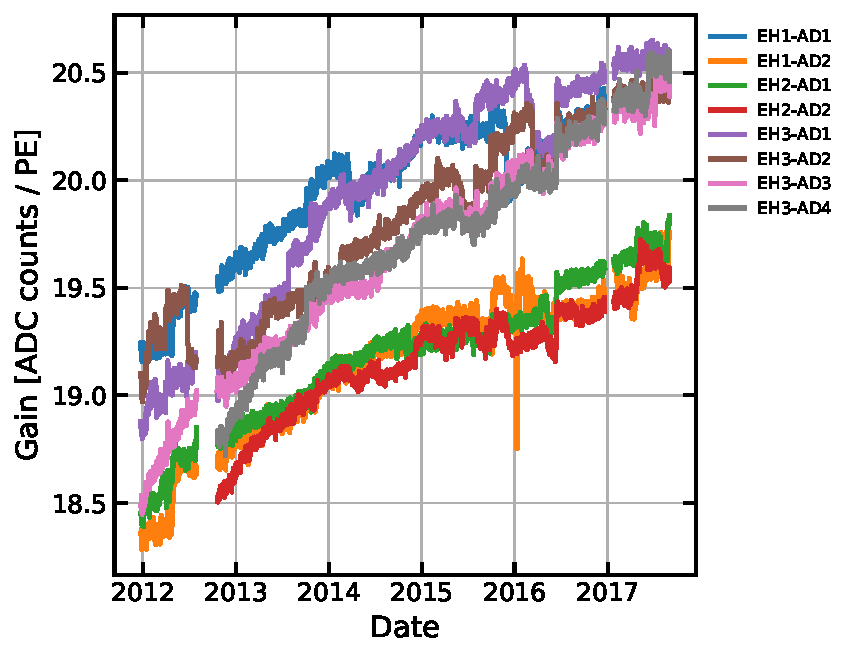
\includegraphics[width=0.8\textwidth]{ch_calibration/gains}
    \caption[PMT gains over time]{PMT gains over time, as measured by the rolling gain.}
    \label{fig:gain}
\end{figure}


\section{Light yield calibration}
\label{sec:light_yield_calib}

The light yield characterized the average
number of photoelectrons (PEs) observed by PMTs
per energy deposited in the liquid scintillator
by a physics event.
It was measured both by deploying the \isotope[60]{Co} calibration source
during weekly calibrations
and using a rolling method based on muon-induced spallation neutron
captures on Gd (nGd), which accumulated sufficient statistics
approximately once per day at the near halls and once per week at the far hall.

Spallation neutrons were produced by muon interactions in the rock,
water, and steel surrounding the ADs.
When these neutrons penetrated into the GdLS,
they captured on a Gd nucleus, leading to the emission of $\gamma$-rays
with energy totalling either \SI{7.95}{\MeV} or \SI{8.54}{\MeV},
depending on the specific isotope of Gd.
Spallation neutrons were identified by searching for events
with energy between \SIlist{6;12}{\MeV} shortly after muon signals.
A background dataset was obtained with an offset time window
and subtracted from the energy distribution of the spallation neutron dataset.
The peaks from the two different isotopes overlapped,
so the distribution was then fit with a double Crystal Ball function.
The (single) Crystal Ball function has the form
\begin{equation}\label{eq:crystal_ball}
    f_\text{CB}(E;\alpha, n, E_0, \sigma) = N \times \begin{cases}
        \exp\left(-\frac{(E-E_0)^2}{2\sigma^2}\right),
            & \frac{E-E_0}{\sigma} > -\alpha \\
        \left(\frac{n}{|\alpha|}\right)^n \exp\left(-\frac{|\alpha|^2}{2}\right)
        \left(\frac{n}{|\alpha|} - |\alpha| - \frac{E-E_0}{\sigma}\right)^{-n},
            & \frac{E-E_0}{\sigma} \leq -\alpha
    \end{cases}
\end{equation}
where $E_0$ represents the peak energy,
$\sigma$ is the resolution of the energy measurement,
$n$ describes the power law for the low-energy tail,
and $\alpha$ gives the location of the transition from peak to tail \cite{cbfunction}.
\Cref{fig:lightyield} shows the light yield over time,
as measured by the spallation neutron captures.

The location of the lower $\gamma$-ray peak (in PE)
was defined to represent \SI{7.95}{\MeV} in reconstructed energy.
Events with other energies were assigned reconstructed energies
based on an assumed linear relation between the measured charge
and the total energy.
Deviations from this assumption of absolute energy linearity were studied;
the energy nonlinearity is discussed in \cref{subsec:abs_energyscale}.

\begin{figure}
    \centering
    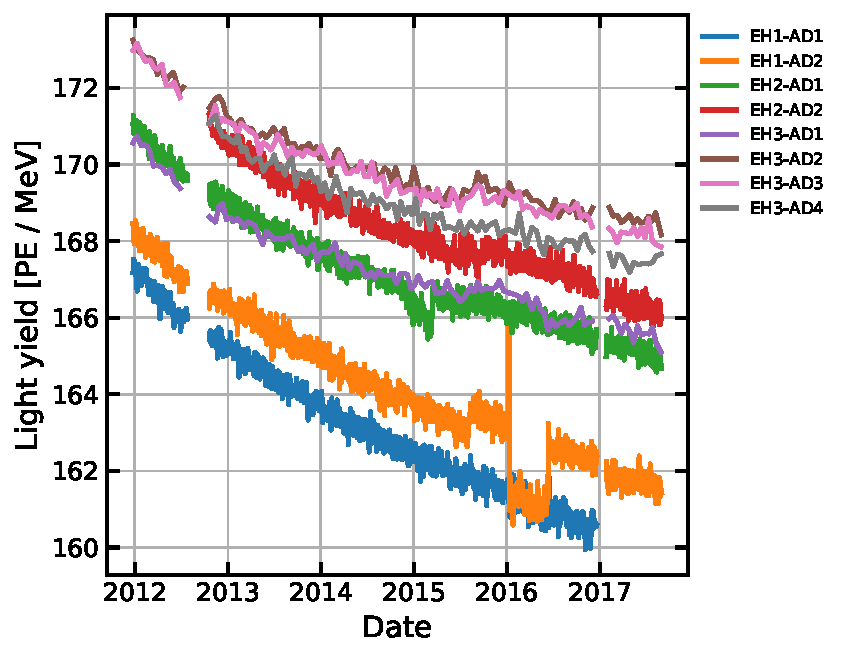
\includegraphics[width=0.8\textwidth]{ch_calibration/light_yield}
    \caption[Light yield over time]{
        Light yield over time, as measured by the spallation neutron method.
        The light yield was measured less frequently in EH3
        because of the lower rate of spallation neutron events
        due to a smaller muon flux.
    }
    \label{fig:lightyield}
\end{figure}

An independent light yield calibration was performed
using the \isotope[60]{Co} calibration source
deployed during the weekly calibration runs.
The \SI{2.506}{\MeV} total energy in $\gamma$-rays emitted by \isotope[60]{Co} decay
provided the reference value for this alternate calibration.
The light yield obtained from this calibration
was different from the spallation neutron--based light yield
due to the absolute energy nonlinearity.
For this thesis, the spallation neutron--based light yield was used
for all reconstructed energy values.

\section{Time calibration}
\label{sec:time_calib}

The times returned by the TDC for each AD must be corrected
to account for differences in cable length as well as
manufacturing differences that could affect the PMT and TDC response times.
Calibration corrections were determined using the LED source.
Each pulse of the LED was synchronized with a calibration trigger so that all PMTs were read out.
The TDC value from each PMT was then converted to time using the
TDC time step value of \SI{1.5625}{\ns} and adjusted
to account for the expected time of flight
of a photon produced in the center of the AD (where the LED was located)
to the given PMT.
After this adjustment, all PMTs should agree on the time of the LED pulse.
The time calibration correction was then computed
as the difference between an individual PMT's hit time
(adjusted for time of flight)
and the known pulse time of the LED.

\section{Special calibration runs}
\label{sec:special_calib}

A variety of special calibration runs were performed
to address specific questions which arose during operation of the experiment.
During the Summer 2012 shutdown for the installation of EH2-AD2 and EH3-AD4,
a special calibration was performed to characterize the correlated background
due to the \amc{} calibration sources.
The \amc{} background and the special calibration are described in \cref{subsec:amc}.
Separately, a special calibration system was temporarily installed in EH1-AD1.
within the AD.
During the December 2016/January 2017 shutdown for the decommissioning of EH1-AD1,
two special calibrations were performed in that AD \cite{calib_proposal2017}.

The special calibration system installed in EH1-AD1 during the Summer 2012 shutdown
allowed calibration sources to be deployed to arbitrary positions,
and was known as the manual calibration system (MCS) \cite{mcs}.
This system consisted of a central rod which could be raised, lowered and rotated,
and a perpendicular arm at the bottom, along which the calibration source
could be moved to reach different radial positions,
as shown in \cref{fig:mcs}.
The MCS was deployed with two calibration sources:
\isotope[60]{Co}, to provide a reference for comparisons with the ACU measurements,
and \isotope[238]{Pu}-\isotope[13]{C} to produce neutrons
and \SI{6.13}{\MeV} $\gamma$-rays.
Results from deploying the MCS at over 1700 positions were used
to measure the detector uniformity \cite{mcs_uniformity}
and neutron capture efficiency \cite{mcs_eff}
and to characterize the position reconstruction (described in \cref{sec:reco_position}).

\begin{figure}
    \centering
    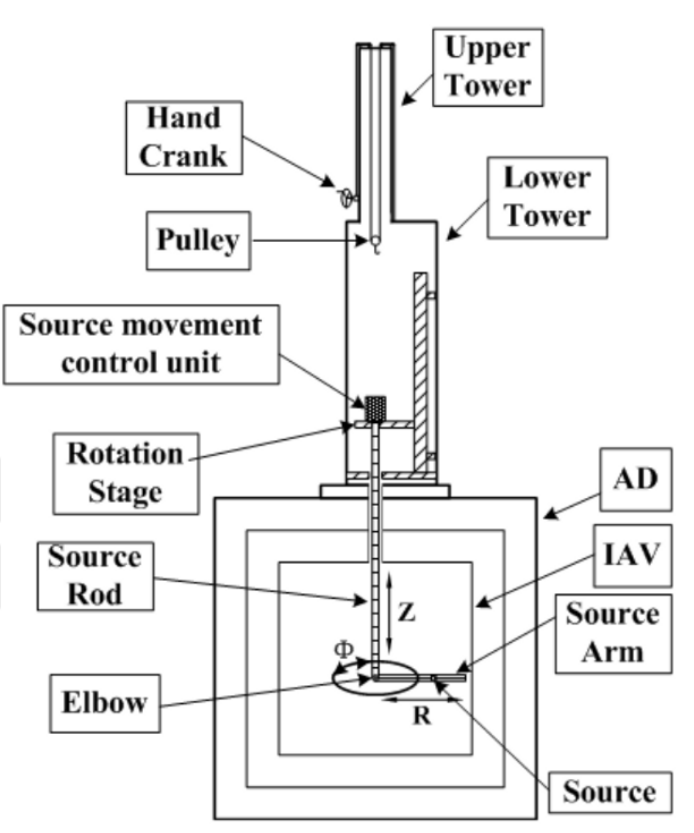
\includegraphics[height=0.34\textheight]{ch_calibration/mcs}
    \caption[Manual calibration system]{
        Schematic diagram of the manual calibration system (MCS) during deployment.
    }
    \label{fig:mcs}
\end{figure}

The first special calibration of the Winter 2016-2017 shutdown
examined the impact of optical shadowing,
when the calibration source enclosures and cable weights
absorbed a small fraction of the scintillation light
produced during calibration-related events,
thus biasing the apparent energy deposited during a calibration event,
as depicted in \cref{fig:optical_shadowing}.
For the special calibration run,
a reflective PTFE enclosure (estimated reflectivity \SI{100}{\percent})
was used for the \isotope[60]{Co} source
instead of the usual stainless steel (estimated reflectivity \SI{45}{\percent}).
Additionally, the bottom weight was removed
so that it would not impact the measurement via additional shadowing.
The calibration run determined that
the optical shadowing effect biased the light yield by \SI{\sim0.6}{\percent}.
This correction was included in the light yield computations.

\begin{figure}
    \centering
    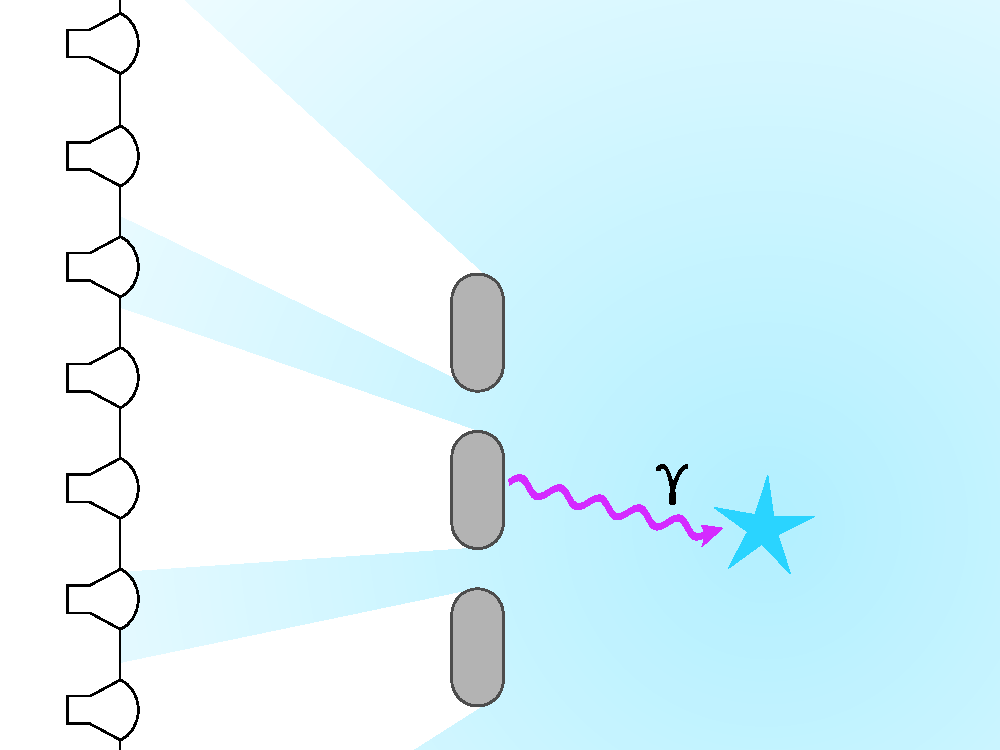
\includegraphics[width=0.5\textwidth]{ch_calibration/optical_shadow}
    \caption[Optical shadowing diagram]{
        Diagram showing optical shadowing, not to scale.
        The top and bottom capsule shapes represent the weights
        which kept the source enclosure (middle capsule) aligned.
        The capsules were connected with a PTFE-jacketed stainless steel cable (not shown).
        The star represents an energy deposition in the liquid scintillator,
        for example Compton scattering or $e^+e^-$ pair production.
        The true effect of optical shadowing was approximately \SI{0.6}{\percent}.
    }
    \label{fig:optical_shadowing}
\end{figure}

The second Winter 2016-2017 special calibration run
was a measurement of the absolute efficiency for neutron capture on Gd.
Additional neutron emitters
(higher-activity \amc{} as well as \isotope[241]{Am}-\isotope[9]{Be})
were deployed along all three ACU axes,
and the resulting neutron detection efficiency
was \SI{81.48\pm0.74}{\percent},
with the uncertainty reduced from a previous value of \SI{1.69}{\percent}.
The analysis presented in this thesis
relied on neutron captures on hydrogen (nH),
so full details of the calibration procedure and determination of the efficiency
will be left to \cite{reactor_flux2019}.

\section{Channel quality}
\label{sec:channel_quality}

Occasionally one or more components of the PMT high voltage power supply
or data readout malfunctioned or produced degraded signals,
leading to a substantial change in measured PMT gain.
Anomalous gain readings were flagged during weekly data quality checks,
and any problematic PMTs were disabled.
Usually at most one PMT at a time was affected in any AD.
The most common problem was a degraded high voltage supply,
and was fixed by replacing the high voltage module.
When any of the PMTs was disabled, the calorimetric response of the ADs
was slightly altered.
In particular, the number of photoelectrons collected
decreased by $n/192$ (on average),
relative to a configuration with \num{192} functioning PMTs,
with $n$ representing the number of disabled PMTs.
A correction was applied to the light yield to compensate for this average behavior.

